\section{The drag force term}
We start by the drag force term. 
Our simulations reach a quasi steady regime meaning that we can consider the velocities of the particular phase and fluid phase as constant.
Now lat's place our selves in the reference frame moving at the averaged velocity of the particles. 
In this frame of reference the particles are thus fixed and see the fluid flowing through, experiencing a drag force due to the stress on the droplets surface. 
Therefore, in this referential considering $\pavg{\textbf{u}} = \textbf{0}$, the momentum equation \ref{eq:homo_momentum_p} yields, 
\begin{equation*}
    m_\alpha \nablab \cdot \left(\pavg{\textbf{u}_\alpha' \textbf{u}_\alpha'}\right). 
    = \pavg{\int_{V_\alpha} \textbf{b} dS}
    + \pavg{\int_{S_\alpha} \textbf{T}_c  \cdot \textbf{n}_c dS}
\end{equation*}
\tb{to be disscused}
We can observe that the divergence of the fluctuation is balanced by the two contributions to the RHS.  
Besides, the body force term has the simple expression, $\pavg{\int_{V_\alpha} \textbf{b} dV} = - nV_\alpha (\rho_d-\rho_c) \textbf{g}$. 
Therefore, the drag force term must be expressed as the sum of a pure drag force which balance the body force and a divergence of a stress which balance in this can the Reynolds stress \citep{zhang2021ensemble,wang2021numerical,nott2011suspension}. 
In this section we focus on the pure drag component and expresses it in the dimensionless form such as, 
\begin{align*}
    \pnavg{F_\mu}
    = \frac
    {\pnavg{\int_{V_\alpha} \textbf{T}\cdot \textbf{n}dV}}
    {\mu_c U D}
    = \frac
    {\left(\rho_d -\rho_c\right) \textbf{g}}
    {\mu_c U}D^2
\end{align*}
Where $\pnavg{F_\mu}$ is the pure dimensionless drag force along the direction of the velocity. 

\ref{fig:f_mu} displays the interphase drag force for different \textit{Galileo} number and volume fraction. 
\begin{figure}[h!]
    \centering
    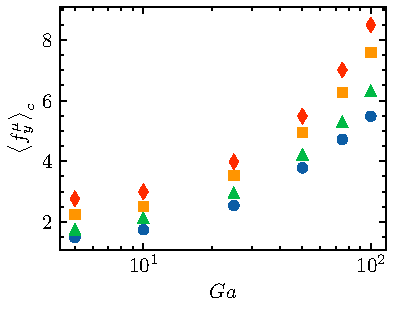
\includegraphics[height=0.3\textwidth]{image/HOMOGENEOUS/fCA/FH_mu_Ga.pdf}
    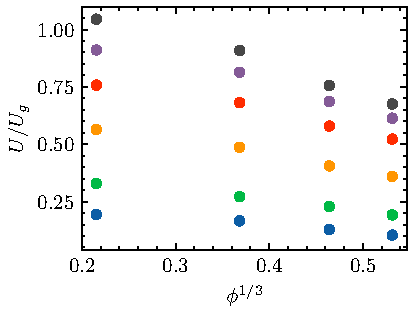
\includegraphics[height=0.3\textwidth]{image/HOMOGENEOUS/fCA/UstokesGa.pdf}
    \caption{(left) Dimensionless drag forces in terms of the \textit{Galileo} number for different volume fraction $\phi$. The other parameters are fixed at $\rho_r = 1.11$, $\mu_r = 0.1$ and $Bo = 1$.
    (dots) Numerical simulations, 
    (dashed line) empirical formula \ref{eq:f_mu_scaling}.
    (right) Dimensionless drift velocity.}
    \label{fig:f_mu}
\end{figure}
Based on the numerical results we could find simple scaling for the drag force at moderate inertial regime. 
Indeed, it yields,
\begin{equation}
    \cavg{F^\mu} = e^{5.66 \phi^{1/3}}  Ga^{0.33} 0.59 + Ga^{0.92} +18.29
    \label{eq:f_mu_scaling}
\end{equation}
From \ref{fig:f_mu} and \ref{eq:f_mu_scaling} it is evident  that in low inertial regime, the drag force scales as $f \sim Ga^{0.33}$ regardless of the volume fraction. 
Regarding the dependency of the force with $\phi$, we observe that the logarithms of the force is proportional $\phi^{1/3}$. 
This reminds the scaling of \cite{sangani1987sedimentation} which found the same $\phi$'s dependency, but on the drift velocity of arranged bubbles arrays.
This scaling is illustrated \ref{fig:f_mu} (right) where we can see that the drift velocity is indeed proportional to $\phi^{1/3}$ regardless of the \textit{Galileo} number.  